\documentclass{article}
\usepackage{fullpage}
\usepackage{amssymb}
\usepackage{amsmath}
\usepackage[utf8]{inputenc}
\usepackage{mathtools}

% Theorems
\usepackage{amsthm}
\renewcommand\qedsymbol{$\blacksquare$}
\makeatletter
\@ifclassloaded{article}{
    \newtheorem{definition}{Definition}[section]
    \newtheorem{example}{Example}[section]
    \newtheorem{theorem}{Theorem}[section]
    \newtheorem{corollary}{Corollary}[theorem]
    \newtheorem{lemma}{Lemma}[theorem]
}{
}
\makeatother

% Random Stuff
\setlength\unitlength{1mm}

\newcommand{\insertfig}[3]{
\begin{figure}[htbp]\begin{center}\begin{picture}(120,90)
\put(0,-5){\includegraphics[width=12cm,height=9cm,clip=]{#1.eps}}\end{picture}\end{center}
\caption{#2}\label{#3}\end{figure}}

\newcommand{\insertxfig}[4]{
\begin{figure}[htbp]
\begin{center}
\leavevmode \centerline{\resizebox{#4\textwidth}{!}{\input
#1.pstex_t}}
\caption{#2} \label{#3}
\end{center}
\end{figure}}

\long\def\comment#1{}

\newcommand\norm[1]{\left\lVert#1\right\rVert}
\DeclareMathOperator*{\argmin}{arg\,min}
\DeclareMathOperator*{\argmax}{arg\,max}

% bb font symbols
\newfont{\bbb}{msbm10 scaled 700}
\newcommand{\CCC}{\mbox{\bbb C}}

\newfont{\bbf}{msbm10 scaled 1100}
\newcommand{\CC}{\mbox{\bbf C}}
\newcommand{\PP}{\mbox{\bbf P}}
\newcommand{\RR}{\mbox{\bbf R}}
\newcommand{\QQ}{\mbox{\bbf Q}}
\newcommand{\ZZ}{\mbox{\bbf Z}}
\renewcommand{\SS}{\mbox{\bbf S}}
\newcommand{\FF}{\mbox{\bbf F}}
\newcommand{\GG}{\mbox{\bbf G}}
\newcommand{\EE}{\mbox{\bbf E}}
\newcommand{\NN}{\mbox{\bbf N}}
\newcommand{\KK}{\mbox{\bbf K}}
\newcommand{\KL}{\mbox{\bbf KL}}
\newcommand{\II}{\mbox{\bbf I}}

% Vectors
\renewcommand{\aa}{{\bf a}}
\newcommand{\bb}{{\bf b}}
\newcommand{\cc}{{\bf c}}
\newcommand{\dd}{{\bf d}}
\newcommand{\ee}{{\bf e}}
\newcommand{\ff}{{\bf f}}
\renewcommand{\gg}{{\bf g}}
\newcommand{\hh}{{\bf h}}
\newcommand{\ii}{{\bf i}}
\newcommand{\jj}{{\bf j}}
\newcommand{\kk}{{\bf k}}
\renewcommand{\ll}{{\bf l}}
\newcommand{\mm}{{\bf m}}
\newcommand{\nn}{{\bf n}}
\newcommand{\oo}{{\bf o}}
\newcommand{\pp}{{\bf p}}
\newcommand{\qq}{{\bf q}}
\newcommand{\rr}{{\bf r}}
\renewcommand{\ss}{{\bf s}}
\renewcommand{\tt}{{\bf t}}
\newcommand{\uu}{{\bf u}}
\newcommand{\ww}{{\bf w}}
\newcommand{\vv}{{\bf v}}
\newcommand{\xx}{{\bf x}}
\newcommand{\yy}{{\bf y}}
\newcommand{\zz}{{\bf z}}
\newcommand{\0}{{\bf 0}}
\newcommand{\1}{{\bf 1}}

% Matrices
\newcommand{\Ab}{{\bf A}}
\newcommand{\Bb}{{\bf B}}
\newcommand{\Cb}{{\bf C}}
\newcommand{\Db}{{\bf D}}
\newcommand{\Eb}{{\bf E}}
\newcommand{\Fb}{{\bf F}}
\newcommand{\Gb}{{\bf G}}
\newcommand{\Hb}{{\bf H}}
\newcommand{\Ib}{{\bf I}}
\newcommand{\Jb}{{\bf J}}
\newcommand{\Kb}{{\bf K}}
\newcommand{\Lb}{{\bf L}}
\newcommand{\Mb}{{\bf M}}
\newcommand{\Nb}{{\bf N}}
\newcommand{\Ob}{{\bf O}}
\newcommand{\Pb}{{\bf P}}
\newcommand{\Qb}{{\bf Q}}
\newcommand{\Rb}{{\bf R}}
\newcommand{\Sb}{{\bf S}}
\newcommand{\Tb}{{\bf T}}
\newcommand{\Ub}{{\bf U}}
\newcommand{\Wb}{{\bf W}}
\newcommand{\Vb}{{\bf V}}
\newcommand{\Xb}{{\bf X}}
\newcommand{\Yb}{{\bf Y}}
\newcommand{\Zb}{{\bf Z}}

% Calligraphic
\newcommand{\Ac}{{\cal A}}
\newcommand{\Bc}{{\cal B}}
\newcommand{\Cc}{{\cal C}}
\newcommand{\Dc}{{\cal D}}
\newcommand{\Ec}{{\cal E}}
\newcommand{\Fc}{{\cal F}}
\newcommand{\Gc}{{\cal G}}
\newcommand{\Hc}{{\cal H}}
\newcommand{\Ic}{{\cal I}}
\newcommand{\Jc}{{\cal J}}
\newcommand{\Kc}{{\cal K}}
\newcommand{\Lc}{{\cal L}}
\newcommand{\Mc}{{\cal M}}
\newcommand{\Nc}{{\cal N}}
\newcommand{\Oc}{{\cal O}}
\newcommand{\Pc}{{\cal P}}
\newcommand{\Qc}{{\cal Q}}
\newcommand{\Rc}{{\cal R}}
\newcommand{\Sc}{{\cal S}}
\newcommand{\Tc}{{\cal T}}
\newcommand{\Uc}{{\cal U}}
\newcommand{\Wc}{{\cal W}}
\newcommand{\Vc}{{\cal V}}
\newcommand{\Xc}{{\cal X}}
\newcommand{\Yc}{{\cal Y}}
\newcommand{\Zc}{{\cal Z}}

% Bold greek letters
\newcommand{\alphab}{\hbox{\boldmath$\alpha$}}
\newcommand{\betab}{\hbox{\boldmath$\beta$}}
\newcommand{\gammab}{\hbox{\boldmath$\gamma$}}
\newcommand{\deltab}{\hbox{\boldmath$\delta$}}
\newcommand{\etab}{\hbox{\boldmath$\eta$}}
\newcommand{\lambdab}{\hbox{\boldmath$\lambda$}}
\newcommand{\epsilonb}{\hbox{\boldmath$\epsilon$}}
\newcommand{\nub}{\hbox{\boldmath$\nu$}}
\newcommand{\mub}{\hbox{\boldmath$\mu$}}
\newcommand{\zetab}{\hbox{\boldmath$\zeta$}}
\newcommand{\phib}{\hbox{\boldmath$\phi$}}
\newcommand{\psib}{\hbox{\boldmath$\psi$}}
\newcommand{\thetab}{\hbox{\boldmath$\theta$}}
\newcommand{\taub}{\hbox{\boldmath$\tau$}}
\newcommand{\omegab}{\hbox{\boldmath$\omega$}}
\newcommand{\xib}{\hbox{\boldmath$\xi$}}
\newcommand{\sigmab}{\hbox{\boldmath$\sigma$}}
\newcommand{\pib}{\hbox{\boldmath$\pi$}}
\newcommand{\rhob}{\hbox{\boldmath$\rho$}}

\newcommand{\Gammab}{\hbox{\boldmath$\Gamma$}}
\newcommand{\Lambdab}{\hbox{\boldmath$\Lambda$}}
\newcommand{\Deltab}{\hbox{\boldmath$\Delta$}}
\newcommand{\Sigmab}{\hbox{\boldmath$\Sigma$}}
\newcommand{\Phib}{\hbox{\boldmath$\Phi$}}
\newcommand{\Pib}{\hbox{\boldmath$\Pi$}}
\newcommand{\Psib}{\hbox{\boldmath$\Psi$}}
\newcommand{\Thetab}{\hbox{\boldmath$\Theta$}}
\newcommand{\Omegab}{\hbox{\boldmath$\Omega$}}
\newcommand{\Xib}{\hbox{\boldmath$\Xi$}}

% mixed symbols
\newcommand{\sinc}{{\hbox{sinc}}}
\newcommand{\diag}{{\hbox{diag}}}
\renewcommand{\det}{{\hbox{det}}}
\newcommand{\trace}{{\hbox{tr}}}
\newcommand{\tr}{\trace}
\newcommand{\sign}{{\hbox{sign}}}
\renewcommand{\arg}{{\hbox{arg}}}
\newcommand{\var}{{\hbox{var}}}
\newcommand{\cov}{{\hbox{cov}}}
\renewcommand{\Re}{{\rm Re}}
\renewcommand{\Im}{{\rm Im}}
\newcommand{\eqdef}{\stackrel{\Delta}{=}}
\newcommand{\defines}{{\,\,\stackrel{\scriptscriptstyle \bigtriangleup}{=}\,\,}}
\newcommand{\<}{\left\langle}
\renewcommand{\>}{\right\rangle}
\newcommand{\Psf}{{\sf P}}
\newcommand{\T}{\top}
\newcommand{\m}[1]{\begin{bmatrix} #1 \end{bmatrix}}

% more stuff
\newcommand{\ev}[2]{\Big|_{#1}^{#2}}
\newcommand{\evv}[2]{\Big|_{#1}^{#2}}
\newcommand{\set}[1]{\left\{#1\right\}}
\newcommand{\s}[1]{\sqrt{#1}}
\newcommand{\f}[2]{\frac{#1}{#2}}
\newcommand{\p}[2]{\frac{\partial #1}{\partial #2}}
\providecommand{\t}[1]{\text{#1}}
\providecommand{\span}[1]{\text{span}\left(#1\right)}
\providecommand{\set}[1]{\left\{#1\right\}}
\providecommand{\l}[0]{\left}
  \providecommand{\r}[0]{\right}
\newcommand{\bm}[1]{\begin{bmatrix}#1\end{bmatrix}}
\renewcommand{\bf}[1]{\mathbf{#1}}
\newcommand{\pn}[1]{\left( #1 \right)}
\newcommand{\abs}[1]{\left| #1 \right|}
\newcommand{\bk}[1]{\left[ #1 \right]}
\newcommand{\cis}[1]{\pn{\cos\pn{#1} + i\sin\pn{#1}}}
\newcommand{\cisi}[1]{\pn{\cos\pn{#1} - i\sin\pn{#1}}}
\renewcommand{\Im}[1]{\text{Im}\pn{#1}}
\renewcommand{\Re}[1]{\text{Re}\pn{#1}}
\newcommand{\subproblem}[1]{\noindent(#1)}

\makeatletter
\renewcommand*\env@matrix[1][*\c@MaxMatrixCols c]{%
  \hskip -\arraycolsep
  \let\@ifnextchar\new@ifnextchar
  \array{#1}}
\makeatother



\begin{document}

\section{Shrinkage Methods}
Shrinkage methods are continuous method for retaining a subset of the predictors and discarding the rest.
The shrinkage methods don't suffer much from high variability.

\subsection{Ridge Regression}
The ridge coefficients minimize a penalized residual sum of squares,
\begin{equation}
  \label{eq:ridge}
  \hat{\beta}^\text{ridge} = \argmin_\beta \left\{ \sum_{i=1}^{N}\left( y_i - \beta_0 - \sum_{j=1}^{p}x_{ij}\beta_j\right)^2  + \lambda \sum_{j=1}^{p}\beta_j^2\right\}.
\end{equation}
An equivalent way to write the ridge problem is
\begin{equation}
\begin{split}
  \hat{\beta}^\text{ridge} &= \argmin_\beta \sum_{i=1}^{N}\left( y_i - \beta_0 - \sum_{j=1}^{p}x_{ij}\beta_j\right)^2, \\
  &\text{subject to} \sum_{j=1}^{p}\beta_j^2 \le t,
\end{split}
\end{equation}
which makes explicit the size constraint on the parameters. To find the solution of the ridge regression, we rewrite the equality in (\ref{eq:ridge}) in matrix form,
\begin{equation}
  \label{eq:ridge_matrix_form}
  \text{RSS}\pn{\lambda} = \pn{\yy - \Xb \beta}^\top \pn{\yy - \Xb \beta} + \lambda \beta^\top \beta. 
\end{equation}
Taking the gradient of (\ref{eq:ridge_matrix_form}), we are able to see that the ridge regression solutions are
\begin{equation}
  \label{eq:ridge_solution}
  \hat{\beta}^\text{ridge} = \pn{\Xb^\top \Xb + \lambda \Ib}^{-1} \Xb^\top \yy,
\end{equation}
where $\Ib$ is the $p \times p$ identity matrix.

\paragraph{Ridge Regression as a Posterior Distribution} Suppose $y_i \sim \mathcal{N}\pn{\beta_0 +x_i^\top \beta, \sigma^2}$, and the parameters $\beta_j$ are each distributed as $\mathcal{N}\pn{0,\tau^2}$, independently of one another. Thenm, the neagative log-posterior density of $\beta$, with $\tau^2$ and $\sigma^2$ assumed known, is equal to the expression in (\ref{eq:ridge_matrix_form}), with $\lambda = \sigma^2/\tau^2$. Thus, in other words, the ridge estimate is the mode of the posterior distribution; since the distribution is Gaussian, it is also the posterior mean.

\subsection{The Lasso}
The \text{lasso} is a shrinkage method like ridge, with subtle but imporant differences. The lasso estimate is defined by
\begin{equation}
  \begin{split}
  \hat{\beta}^\text{lasso} &= \argmin_\beta \sum_{i=1}^{N}\pn{y_i - \beta_0 - \sum_{j=1}^{p}x_{ij}\beta_j}^2 \\
  &\text{subject to} \sum_{j=1}^{p}|\beta_j| \le t.
  \end{split}
\end{equation}
We can also write the lasso problem in the equivalent \textit{Lagrangian form}
\begin{equation}
  \label{eq:lasso}
  \hat{\beta}^\text{lasso} = \argmin_\beta \left\{ \f{1}{2}\sum_{i=1}^{N}\pn{y_i - \beta_0 - \sum_{j=1}^{p}x_{ij}\beta_j}^2  + \lambda \sum_{j=1}^{p}|\beta_j|\right\} .
\end{equation}
Computing the lasso solution is a quadratic programming problem. Because of the nature of the constraint, making $t$ sufficiently small will cause some of the coefficients to be exactly zero. Thus, the lasso does a kind of continuous subset selection. If $t$ is chosen larger than $t_0 = \sum_{j=1}^{p}|\hat{\beta}_j|$ (where $\hat{\beta}_j = \hat{\beta}_j^\text{lasso}$, the least squares estimates), then the lasso estimates are the $\hat{\beta}_j$'s.

\subsection{Discussion: Subset Selection, Ridge Regrssion and the Lasso}
In this subsection, we will discuss and compare three approaches for restricting linear regression model. In the case of an orthonormal input matrix $\Xb$ the three procedures have explicit solutions. Ridge regression does a proportional shrinkage. Lasso translates each coefficient by a constant factor $\lambda$, truncating at zero. This is called ``soft thresholding,'' and is used in the context of wavelet-based smoothing. Best-subset selection drops all variables with coefficient smaller than the $M$th largest; this is a form of ``hard thresholding.''

For the nonorthogonal case,
\begin{center}
  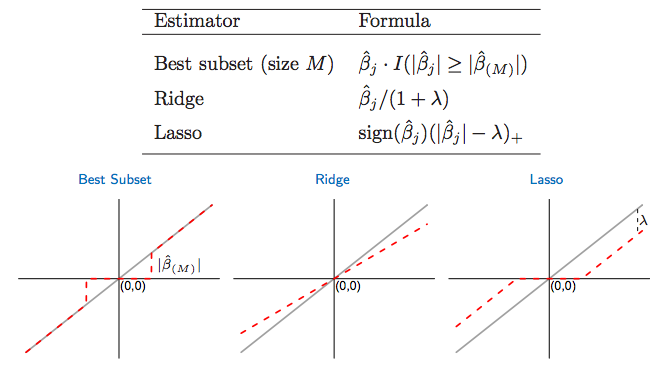
\includegraphics[scale=0.5]{assets/linear_regression_estimator} \\
  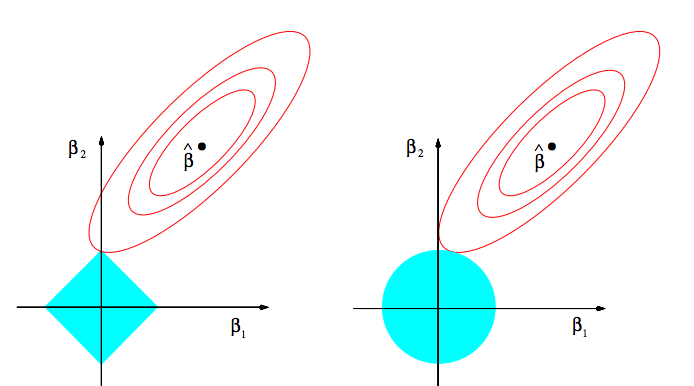
\includegraphics[scale=0.5]{assets/ridge_and_lasso}
\end{center}
From the diagram above, it suggests that lasso tends to give a sparser solution.

\section{Linear Methods for Classification}
In this section, we'll discuss about the classification problem using linear methods.  We require some monotone transformation of $\delta_k$ or $\text{Pr}(G = k | X = x)$ be linear for the decision boundaries to be linear. For example, if htere are two cases, a popular model for the posterior probabilities is
\begin{equation}
  \begin{split}
    \text{Pr}(G = 1 | X = x) &= \f{\text{exp}\pn{\beta_0 + \beta^\top x}}{ 1 + \text{exp}\pn{\beta_0 + \beta^\top x}}, \\
    \text{Pr}(G = 2 | X = x) &= \f{1}{1 + \text{exp}\pn{\beta_0 + \beta^\top x}}.
  \end{split}
\end{equation}
Here the monotone transformation is the \textit{logit} transformation: $\log [p/(1-p)]$, and in fact we see that
\begin{equation}
  \log \f{\text{Pr}(G = 1 | X = x)}{\text{Pr}(G = 2 | X = x)} = \beta_0 + \beta^\top x.
\end{equation}
The decision boundary is the set of points for which the log-odds are zero, and this is a hyperplane defined by $\{x | \beta_0 + \beta^\top x\}$. We provide two popular methods that result in linear log-odds or logits: linear discriminant analysis and linear logistic regrssion.

\subsection{Linear Discriminant Analysis}
Suppose $f_k(x)$ is the class-conditional density of $X$ in class $G = k$, and let $\pi_k$ be the prior probability of class $k$, with $\sum_{k=1}^{K}\pi_k = 1$. A simple application of Bayes theorem gives us
\begin{equation}
  \text{Pr}(G = k | X = x) = \f{f_k(x)\pi_k}{\sum_{l=1}^{K}f_l(x) \pi_l}.
\end{equation}
Suppose that we model each class density as multivariate Gaussian:
\begin{equation}
  \label{eq:multivariate_gaussian}
  f_k(x) = \f{1}{\pn{2\pi}^{p/2}|\Sigmab_k|^{1/2}}\text{exp}\pn{-\f{1}{2}\pn{x - \mu_k}^\top \Sigmab_k^{-1} \pn{x - \mu_k}}.
\end{equation}
Linear discriminant analysis (LDA) arises in the special case when we assume that the classes have a common covariance matrix $\Sigmab_k = \Sigmab$ for all $k$. In comparing two classes $k$ and $l$, it is sufficient to look at the log-ratio, and we see that
\begin{equation}
  \begin{split}
    \log \f{\text{Pr}(G = k | X = x)}{\text{Pr}(G = l | X = x)} &= \log \f{f_k(x)}{f_l(x)} + \log \f{\pi_k}{\pi_l} \\
    &= \log \f{\pi_k}{\pi_l} - \f{1}{2} \pn{\mu_k + \mu_l}^\top \Sigmab^{-1} \pn{\mu_k - \mu_l} + x^\top \Sigmab^{-1} \pn{\mu_k - \mu_l}
  \end{split}
\end{equation}


\section{Principal Component Analysis}
Consider a dataset $\mathcal{D}$. We want to find the subspace so we can project $\mathcal{D}$
onto a lower dimensional dataset that accounts for the variance, $\tilde{\mathcal{D}}$.
The process is as follows:
\begin{enumerate}
\item[(a)] Calculate the mean of the dataset $\mathcal{D}$.
  \[
  \mu = \frac{1}{n}\sum_{i=1}^{n}\mathbf{x}_i.
  \]
\item[(b)] Standardize the data.
  \[
  \tilde{\mathbf{x}}_i = \mathbf{x}_i - \mu.
  \]
\item[(c)] Compute the covariance matrix.
  \[
  \mathbf{\Sigma} = \sum_{i}\tilde{\mathbf{x}}_i\tilde{\mathbf{x}}_i^\top = \frac{1}{N}\tilde{X}^\top \tilde{X}.
  \]
\item[(d)] Compute the eigendecomposition of $\mathbf{\Sigma}$.
  \[
  \mathbf{\Sigma} = P\Lambda P^\top
  \]
  where $\Lambda$ is a diagonal matrix of eigenvalues sorted in a decreasing way.
  \item[(e)] Project data onto the eigenvectors corresponding to the top $k$ eigenvectors to get $\mathcal{D}$.
\end{enumerate}


\section{Gaussian Models}
In this chapter, we discuss the multivariate Gaussian which is very popular for calculating the joint probability density function.

The pdf for an multivariate normal (MVN) in $D$ dimensions is defined by
\begin{equation}
  \label{eq:multivariate_normal}
  \mathcal{N}\pn{\xx | \mub, \Sigmab} = \f{1}{\pn{2\pi}^{D/2}|\Sigmab|^{1/2}} \exp\pn{-\f{1}{2}\pn{\xx - \mub}^\top \Sigmab^{-1} \pn{\xx - \mub}}.
\end{equation}
Consider the Mahalanobis distance beteween a data vector $\xx$ and the mean vector $\mub$. Using an eigendecomposition of $\Sigmab$, we could write $\Sigmab = \Ub\Lambdab \Ub^\top$, where $\Ub$ is an orthonormal matrix of eigenvalues satisfying $\Ub^\top \Ub = \Ib$, and $\Lambdab$ is a diagonal matrix of eigenvalues. Then, we can find the inverse of covariance matrix as follows:
\begin{equation}
  \Sigmab^{-1} = \pn{\Ub \Lambdab \Ub^\top}^{-1} = \Ub^{-\top}\Lambda^{-1} \Ub^{-1} = \Ub \Lambdab^{-1} \Ub^\top = \sum_{i=1}^{D}\f{1}{\lambda_i}\uu_i \uu_i^\top
\end{equation}
where $\uu_i$ is the $i$th column of $\Ub$, containing the $i$th eigenvector. Now, we can rewrite the Mahalanobis distance as
\begin{equation}
  \label{eq:mahalanobis_distance}
  \begin{split}
    \pn{\xx - \mub}^\top \Sigmab^{-1} \pn{\xx - \mub} &= \pn{\xx - \mub}^\top \pn{\sum_{i=1}^{D} \f{1}{\lambda_i}\uu_i \uu_i^\top } \pn{\xx - \mub} \\
    &= \sum_{i=1}^{D}\f{1}{\lambda_i} \pn{\xx - \mub}^\top \uu_i \uu_i^\top \pn{\xx - \mub} \\
    &= \sum_{i=1}^{D} \f{y_i^2}{\lambda_i}
  \end{split}
\end{equation}
where $y_i = \uu_i^\top \pn{\xx - \mub}$. Notice that the last equality of (\ref{eq:mahalanobis_distance}) is an equaltion of an ellipse in $D$ dimension. In general, we can interpret the Mahalanobis distance as the distance corresponding to Euclidean distance in the transformed coordinate system, where we shift by $\mub$ and rotate by $\Ub$.

\subsection{Gaussian Discriminant Analysis}
One application of Multivariate Normal is to define the class conditional densities in a generative classfier, i.e.,
\begin{equation}
  \text{Pr}\pn{\xx | y = c, \thetab} = \mathcal{N}\pn{\xx | \mub_c, \Sigmab_c}.
\end{equation}
Applying Bayes Rules, one could obtain
\begin{equation}
  \text{Pr}\pn{y = c | \xx, \thetab} = \f{\text{Pr}\pn{\xx | y = c, \thetab}\text{Pr}\pn{y = c | \thetab}}{\sum_{k}\text{Pr}\pn{\xx | y = k, \thetab}\text{Pr}\pn{y = k | \thetab}}.
\end{equation}
Then, we can classify a feature vector by following decision rule:
\begin{equation}
  \label{eq:gda_rule}
  \hat{y}(\xx) = \argmax_c \pn{ \log \text{Pr}\pn{y = c | \pib} + \log \text{Pr}\pn{\xx | \thetab_c}}.
\end{equation}

\subsection{Quadratic Discriminant Analysis}
Plugging in the definition of Multivariate Gaussian, we can obtain the followin equality:
\begin{equation}
  \label{eq:QDA}
  \text{Pr}\pn{y = c | \xx, \thetab} = \f{ \pi_c |2\pi \Sigmab_c |^{-1/2} \exp\pn{-\f{1}{2}\pn{\xx - \mub_c}^\top \Sigmab_c^{-1} \pn{\xx - \mub_c} }}{ \sum_k \pi_k |2\pi \Sigmab_k |^{-1/2} \exp\pn{-\f{1}{2}\pn{\xx - \mub_k}^\top \Sigmab_k^{-1} \pn{\xx - \mub_k} }}.
\end{equation}

\subsection{Linear Discriminant Analysis}
Consider a special case when the covariance matrices are shared across all classes, e.g. $\Sigmab_c = \Sigmab$ for all $c$. In this case, we can further simplify (\ref{eq:QDA}) to
\begin{equation}
  \begin{split}
    \text{Pr}(y = c|\xx, \thetab) &= \f{\pi_c \exp\pn{\mub_c^\top \Sigmab^{-1}\xx - \f{1}{2} \xx^\top \Sigmab^{-1} \xx - \f{1}{2}\mub_c^\top \Sigmab^{-1} \mub_c}}{\sum_k \pi_k \exp\pn{\mub_k^\top \Sigmab^{-1}\xx - \f{1}{2} \xx^\top \Sigmab^{-1} \xx - \f{1}{2}\mub_k^\top \Sigmab^{-1} \mub_k}} \\
    &= \f{\exp\pn{\mub_c^\top \Sigmab^{-1} \xx - \f{1}{2}\mub_c^\top \Sigmab^{-1}\mub_c + \log \pi_c } }{ \sum_k \exp\pn{\mub_k^\top \Sigmab^{-1} \xx - \f{1}{2}\mub_k^\top \Sigmab^{-1}\mub_k + \log \pi_k }}.
  \end{split}
\end{equation}
If we define $\gamma_c = -\f{1}{2}\mub_c^\top \Sigmab^{-1}\mub_c + \log \pi_c$ and $\betab_c = \Sigmab^{-1}\mub_c$, we can further simplify the above equality to
\begin{equation}
  \label{eq:softmax}
  \text{Pr}\pn{y = c | \xx, \thetab} = \f{\exp\pn{ \betab_c^\top \xx + \gamma_c} }{\sum_k \exp\pn{ \betab_k^\top\xx + \gamma_k }}.
\end{equation}
Note that we can further regularize the covariance matrices as follows:
\begin{equation}
  \label{eq:regularized_LDA}
  \hat{\Sigmab} = \lambda \text{diag}\pn{\hat{\Sigmab}_\text{MLE} } + \pn{1 - \lambda}\hat{\Sigmab}_\text{MLE}
\end{equation}
where $\lambda$ controls the amount of regularization.

\subsection{Inference in jointly Gaussian distributions}
Suppose $\xx = \pn{\xx_1, \xx_2}$ is jointly Gaussian with parameters $\mub = \bm{\mub_1 \\ \mub_2}$, $\Sigmab = \bm{\Sigmab_{11} & \Sigmab_{12} \\ \Sigmab_{21} & \Sigmab_{22}}$, and $\Lambdab = \Sigmab^{-1} = \bm{\Lambdab_{11} & \Lambdab_{12} \\ \Lambdab_{21} & \Lambdab_{22}}$. Then, the marginal probabilities are given by
\begin{equation}
  \label{eq:marginal}
  \begin{split}
    p(\xx_1) &= \mathcal{N}\pn{\xx_1 | \mub_1 , \Sigmab_{11}} \\
    p(\xx_2) &= \mathcal{N}\pn{\xx_2 | \mub_2 , \Sigmab_{22}}
  \end{split}
\end{equation}
and the posterior conditional is given by
\begin{equation}
  \label{eq:posterior_MVN}
  \begin{split}
    p\pn{\xx_1 | \xx_2} &= \mathcal{N}\pn{\xx_1 | \mub_{1|2}, \Sigmab_{1|2}} \\
    \mub_{1|2} &= \mub_1 + \Sigmab_{12}\Sigmab_{22}^{-1}\pn{\xx_2 - \mub_2} \\
    \Sigmab_{1|2} &= \Sigmab_{11} - \Sigmab_{12}\Sigmab_{22}^{-1}\Sigmab_{21}
  \end{split}
\end{equation}
The result of (\ref{eq:conditional_MVN}) follows from the Schur's Complement.
  \end{document}

